\section{Selected Materials Specs}
Decision of 2026-11-09: the substrate is Rogers RO3003. Rogers TMM10i is the validation substrate of the simulations. The board thickness is still open (see the PCB table).
\subsection{PCB Substrate -- Rogers RO3003
\label{subsec:selectedPCBsubstrate}}
$$\epsilon_r = 3.00\pm0.04$$
$$\tan \delta = 0.0010$$
\noindent At 10 GHz, 23~$^\circ$C (Rogers RO3000 data sheet). The HFSS model uses $\tan\delta = 0.0013$, the entry of the AEDT library.\par
\noindent Thermal expansion $x/y/z$: $17/16/25$ ppm/$^\circ$C, measured from $-55$ to 288~$^\circ$C; the in-plane value is matched to copper. Thermal conductivity 0.50 W/(m\,K). Neither data sheet gives a value at cryogenic temperature.\par
\noindent Standard thicknesses: 0.127, 0.254, 0.508, 0.762 and 1.524 mm (0.005, 0.010, 0.020, 0.030 and 0.060 in).\par
\textcolor{blue}{\underline{\hyperref[subsec:PCBsubstrateAlt]{Alternatives}}}

\subsection{PCB Substrate -- Rogers TMM10i (validation substrate)
\label{subsec:TMM10i}}
$$\epsilon_r = 9.80\pm0.245$$
$$\tan \delta = 0.0020$$
\noindent Thermal expansion $x/y/z$: $19/19/20$ ppm/K, measured from 0 to 140~$^\circ$C (Rogers TMM data sheet).
\begin{figure}[h]
    \centering
    \vspace{-0.5cm}
    Standard Thicknesses\\
    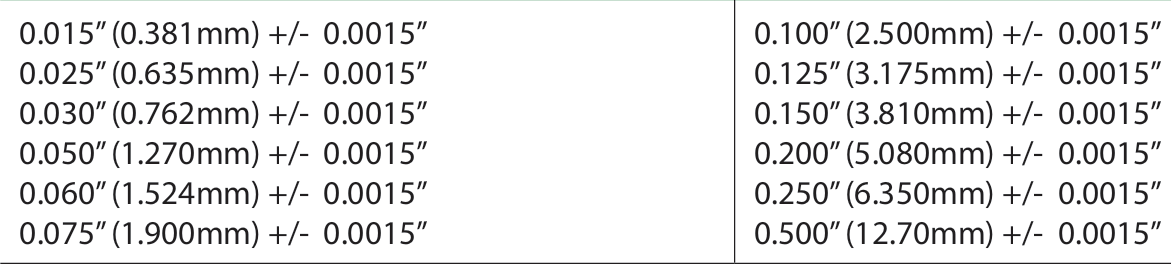
\includegraphics[width=0.5\linewidth]{tex/RogersTTMstandardThicknesses.png}
    \label{fig:RogersTTMstandardThicknesses}
\end{figure}
